\documentclass[12 pt]{article}
\usepackage[letterpaper]{geometry}
\usepackage{times}
\geometry{top=1.5in, bottom=1.0in, left=1.0in, right=1.0in}

\usepackage[hidelinks]{hyperref}
%\renewcommand{\sectionautorefname}{\S}
\usepackage{xcolor}
\hypersetup{
	colorlinks,
	linkcolor={blue!50!black},
	citecolor={blue!50!black},
	urlcolor={blue!80!black}
}


\usepackage{graphicx} %for images
\graphicspath{{images/}}
\usepackage{caption}
\captionsetup[table]{skip=0pt,singlelinecheck=off}
\captionsetup[figure]{skip=0pt,singlelinecheck=off}
\usepackage{subcaption}


\usepackage{booktabs}
\usepackage{enumitem} %customize list numberings

\usepackage[natbibapa]{apacite}
\usepackage{natbib}

\usepackage{tipa}
\newcommand{\nt}[1]{\textipa{[#1]}} % narrow transcription
\newcommand{\wt}[1]{\textipa{/#1/}} % wide transcription


\usepackage{fancyhdr}
\pagestyle{fancy}
\fancyhf{}
\renewcommand{\headrulewidth}{0pt}
\fancyhead[R]{\thepage}

\usepackage{setspace}
\doublespacing

\usepackage{comment}

\newlength\mystoreparindent
\newenvironment{myparindent}[1]{%
	\setlength{\mystoreparindent}{\the\parindent}
	\setlength{\parindent}{#1}
}{%
	\setlength{\parindent}{\mystoreparindent}
}

\usepackage{easyReview}

%-----------------------------

%-----------------------


\title{Supplementary material}
\date{}
\maketitle

\begin{document}
	\bibliographystyle{apacite}

\section*{Participant and demographic information}

Participants were recruited through an open call at the EFL University campus in Hyderabad. Interested volunteers completed a brief language background questionnaire which was used to screen participants as described below. 

As noted in section \ref{bengali_english_in_india}, India has an extremely multilingual an linguistically diverse population. The university campus comprises of students from different parts of the country and world, with varying L1s and different varieties of English. Our aim in screening participants was to minimize between-participant random variability, while maintaining ecological validity considering the actual day-to-day settings in which transfer behaviors likely take place. We chose two metrics to do this: (i) where the participant grew up; and (ii) amount of formal education in Bengali. The first ensures that the variety of Bengali that individuals are exposed to in their surroundings is similar across participants. This would mean that the target representations for Bengali vowels would be expected to be similar. This was especially important because we were not eliciting unilingual L1 Bengali data in this study, and were using an existing data source to estimate the position of Bengali vowels in the formant space. Based on previous literature (c.f. section \ref{asymmetry between sounds}), we expect that L2 vowels shift towards related L1 categories during mixed language utterances. Thus, we wanted to ensure that any between-participant asymmetries in the pattern of shift reflected individual differences in transfer, rather than different acoustic targets. Another reason to control for location was that it is a fairly reliable predictor for language(s) of education, owing to how the education system functions in the country (see Supplementary materials for details).

The second metric is Medium of Instruction (MoI) in school. Most schools in India follow the Three Language Policy, wherein formal education is provided in English, Hindi, and a regional language. \alert{(The idea and implementation of this policy, and its implications for linguistic minorities, has been a matter of much public debate as well as scholarly work; for discussions see, e.g. \cite{tollefson2014language, jhingran2009hundreds, khubchandani1997language, mohanty2009multilingual, ramanathan2005rethinking}).} Sustained formal education in a language is a reliable predictor of LSRW (listening, speaking, reading, writing) skills. Since this study uses written stimuli, we wanted to ensure that all participants were sufficiently comfortable with reading and speaking both Bengali and English, to avoid variability due to reading/task effort.  

Given these considerations, we only recruited participants who had grown up in the state of West Bengal and lived there for the majority of their lives, had parents who both spoke Bengali, and had received at least 5 years of formal education in Bengali (all respondents had received 5+ years of education in English and were pursuing university degrees that are taught in English), and self-reported being proficient in speaking, understanding, and reading Bengali. 

A total of 28 bilingual speakers of Bengali and English (18 female) responded to the recruitment call. Using the inclusion criteria reported above, 10 volunteers (5 female, 5 male, age range 19 to 28) were invited to participate in a speech production study, and were compensated for their time. All participants reported normal hearing, and normal or corrected-to-normal vision. After completion of the study, we followed up with a detailed language background survey at a later date to learn more about the language profiles of the participants. This survey was a modified and consolidated version of three popular bilingualism profiling tools: the Bilingual Language Profile (BLP) \citep{blp}, the Language Experience and Proficiency Questionnaire (LEAP-Q) \citep{leap-q} which incorporates language history and self-assessed proficiency, and the Bilingual Switching Questionnaire (BSWQ) \citep{language_switching_questionnaire}. Together, these incorporate questions about language history, usage, attitudes, and switching experience. \alert{table ... summarizes the key information. The complete questionnaire, along with responses, is available in the ``Data" component of the OSF repository for this project (c.f. section \ref{data_availability}). --footnotes?}

In addition to Bengali and English, all participants reported knowing other languages, the most common being Hindi. Since this situation is representative of the present population and our study concerns only Bengali-English interaction, we only focused on these languages in the survey.
The average age of acquisition was 2.6 for English (range 0 i.e. since birth to 6) and 0.25 (range 0 to 2) for Bengali. Thus, all participants can be described as simultaneous bilinguals, having acquired both English and Bengali at a young age. They report being comfortable using both languages at a young age, with the average being 7.5 for English and 0.3 for Bengali (on a likert scale rating where 0=for as long as I can remember, 5=since I was 5 years old, and so on). As mentioned earlier, all participants had attended schools where Bengali and English were both used as Medium of Instruction (MoI). On average, participants had had more than 16 years (range 7 to 20+) of formal education in English and 11.8 years (range 8 to 15) in Bengali at the time of the study. As described in the inclusion criteria, all participants reported having spent over 15 years in a Bengali-speaking region. At the time of recording, they were living in or around the EFL University campus in Hyderabad, which has a linguistically diverse population. In terms of usage, participants show a range of language usage patterns. Almost 100\% of the participants report exclusively using Bengali with little to no English while interacting with family, and English at school/the workplace. However, language use with friends varies greatly, likely reflecting the language composition of the friend circle. 
The questionnaire asked participants to rate their proficiency in each language. All participants rated themselves as highly proficient in speaking and understanding both Bengali and English. While self-ratings for reading and writing English were at ceiling, ratings for Bengali literacy (reading and writing) showed some variation, with an average of 4.87 (on a 0-6 likert scale, range 3 to 6) for reading and 4.25 (range 3 to 6) for writing. This is a common situation for many educated sections of society, since institutions of higher education beyond the school level largely use English (for discussions about the language politics of higher education in India, see, for example, \cite{mohanty2009multilingual}). 
The language attitude section of the questionnaire reveals interesting insights about the linguistic landscape of the population, and how people experience language in such a setting. When asked how much ``like themselves" participants feel while using each language, response were at ceiling for both languages. Similarly, most participants identified equally strongly with both an ``English-speaking" and a ``Bengali-speaking" culture, possibly because for most people, such linguistic-cultural identities are not clearly delineated and not exclusive of one another. 
These responses shed light on how multiple languages fit seamlessly into different facets of daily life to create a ``continuous" linguistic experience (c.f. ``plurality" as defined by \cite{khubchandani2021plural}). In such a scenario, it is not surprising that language-switching is common, expected, as well as used in creative ways with communicative purpose. Responses to the section on language switching demonstrate this. On average, participants do not report being often unable to recall words in the target language while speaking Bengali (average rating 2.5 on a 1-6 likert scale where 1=never and 6=always) or English (average rating 2.3), indicating that switching is not strictly necessary for filling lexical gaps. Indeed, participants do not report switching between languages without awareness (1.8) or control (1.25). In spite of this, participants report a proclivity to code-switch (rating 3.5). Importantly, a large number of participants report volition while switching languages (4.12), and many report this to be situationally motivated (3.12). These responses indicate that participants are highly aware of their switching habits and move between languages for communicative purposes. This fact, combined with the linguistic situation described here and in section \ref{bengali_english_in_india}, are important to bear in mind while interpreting the results of a transfer study in the present population. 

Given our inclusion criteria, we were able to recruit 10 participants for this study. Although existing studies in the field have used comparable participant numbers, we acknowledge that this is a small sample size. As detailed above, even after a recruitment call that already controlled for language background and education level (recruiting Bengali-English bilinguals in a university campus), we were able to include only 10 out of 28 volunteers (35.7\%) in the final study. Note that the criteria used here establish only a minimal level of between-participant similarity in exposure, dominance, habits, and proficiency, such as is extremely common in most comparable studies. This demonstrates the degree of linguistic variability in the present population. Norms for experimental research on bilingualism have largely been established in a Western context. In settings where linguistic variability at the population level is much greater than these canonically studied groups, establishing comparable levels of experimental control requires significantly greater resources. Given that small sample sizes are likely to have low statistical power, replication with larger sample sizes are important to confirm the observed effects, and provide much-needed data diversity (c.f. discussion in section \ref{introduction}). A more detailed discussion of power analyses in bilingualism research is included as supplementary material on OSF (c.f. section \ref{data_availability}). We hope that this can facilitate more conversation around establishing norms for power and sample size in our field.  



\section*{Supplementary material: power analysis}

Owing to participant availability given our inclusion criteria, we were able to recruit 10 participants for this study (c.f. section Participants in main article). As part of the peer review process, we carried out post-hoc power analyses using the \textit{mixedpower} package \citep{kumle2021estimating} in R. Although there is a body of literature that debates the usefulness of post-hoc power analyses in interpreting the findings of a completed study where statistical analyses have already been performed \citep{lakens_2021,dziak2020interpretation,lenth2007post,gelman2019observed_effect_size}, we have included this section as a discussion around considerations for power calculation in bilingualism research. 

The aim of the analysis was to explore the power of our experiment design to detect the effects we are investigating. The package simulates responses based on a given dataset and runs the specified analyses on these new data, estimating power by calculating how frequently statistical significance is obtained in the simulated data. The target of the analysis was to calculate the power for detecting an effect for our main variables of interest: vowel*context (to test the hypotheses L2-vowels and Asymmetry), and vowel*context*task (to test the hypothesis Paradigm). 

Power is a function of sample size and effect size. Thus, a key issue in power analyses is to estimate the expected effect size for the treatment/factor of interest \citep{brysbaert2018power, kumle2021estimating}. This may be expressed by a variety of measures, including Cohen's d, $\eta ^2$, and model estimates ($\beta$). Using observed effect sizes from the data for power analyses has been shown to be meaningless \citep{hoenig2001abuse, gelman2019observed_effect_size}, since such ``observed power" is a function of the p-value. Therefore, we need a reasonable estimate of effect size. One way to do this is to use effect sizes reported in other existing literature (however, see \cite{brysbaert2018power} who recommends against using effect sizes from single published studies, as these tend to be inflated), or meta analyses. An alternative approach is to define a smallest effect size that is meaningful to us (smallest effect size of interest; SESOI \citep{kumle2021estimating}), and test whether the study has enough power to detect such an effect, if it were to exist. This value needs to be theoretically motivated. To the best of our knowledge, there is no existing literature on typical effect sizes for spectral differences in cross-language vowel production, and not many studies that report effect sizes. Only more discussion in this field will lead to a consensus on what is considered a typical or minimally meaningful cross-language effect. Similarly, while differences between language-switching paradigms have been informally discussed in previous literature, we are not aware of any study that has measured these differences in a controlled experimental setup, and thus no reported effect sizes for between-paradigm differences in phonetic transfer to act as a guideline. 

Cohen \citeyearpar{cohen1988statistical} classifies effect sizes (Cohen's d values) as small ($\leq$0.2), medium (0.5), and large ($\geq$ 0.8). Although the usefulness of this classification has been debated in the literature, these are often used as ballpark values for power analyses in psychological studies (for a discussion, see \cite{brysbaert2018power}). However, this approach does not generalize well to mixed-effects analyses, particularly for complex models with multiple random effects and interactions, as is typical in psycholinguistic and bilingualism research. ``Determining the SESOI for (G)LMMs is difficult in a simulation-based approach where effect sizes are indicated through the model’s unstandardized beta coefficients...relating effect sizes to beta coefficients in complex models is far from trivial and the authors therefore refrain from making specific recommendations. \citep{kumle2021estimating}". 

The results of a power analysis are only as meaningful as the assumptions that go into it. To avoid making arbitrary assumptions, we followed the approach in \cite{brysbaert2018power} (and discussed in \cite{kumle2021estimating}) of extracting the effect sizes from the study of interest and directly modifying all the beta coefficients by a fixed percentage. Note that we are not assuming that doing so gets us closer to a ``true effect size". Instead, we run simulations with a range of effect sizes and report the power of our study to plausibly detect an effect of that size. The results are shown in the plots in figures \ref{figure_power_analysis_f1} and \ref{figure_power_analysis_f2}. Each panel presents power analysis at a different effect size, and is based on 500 simulations. The plots show power (y-axis) over a range of sample sizes (x-axis), given the assumed effect size.   

As expected, power increases as a function of sample size for all effects. However, of greater interest to us is the differences between the power curves in the four panels (a,b,c,d). These demonstrate how results of the power analysis vary as a function of assumed effect size. Note the the range of effect sizes used here is fairly narrow, varying between 15\% smaller and 15\% greater than the observed effect sizes. These differences demonstrate the importance of theoretically justified effect size estimates before attempting to make inferences based on power analyses. This applies equally to aposteriori power analyses done to make decisions about sample sizes prior to data collection (to reiterate, post-hoc power analyses are best avoided). This emphasizes the importance for bilingualism studies to report effect sizes as a part of their results, which can facilitate discussions and meta-analyses that eventually lead to such norms being established in the field. \footnote{Thanks to the anonymous reviewer at BLC for initiating a fruitful discussion around this.}

\newpage
\begin{figure} \label{figure_power_analysis_f1}
	\centering
	\begin{subfigure}[t]{0.8\textwidth}
		\centering
		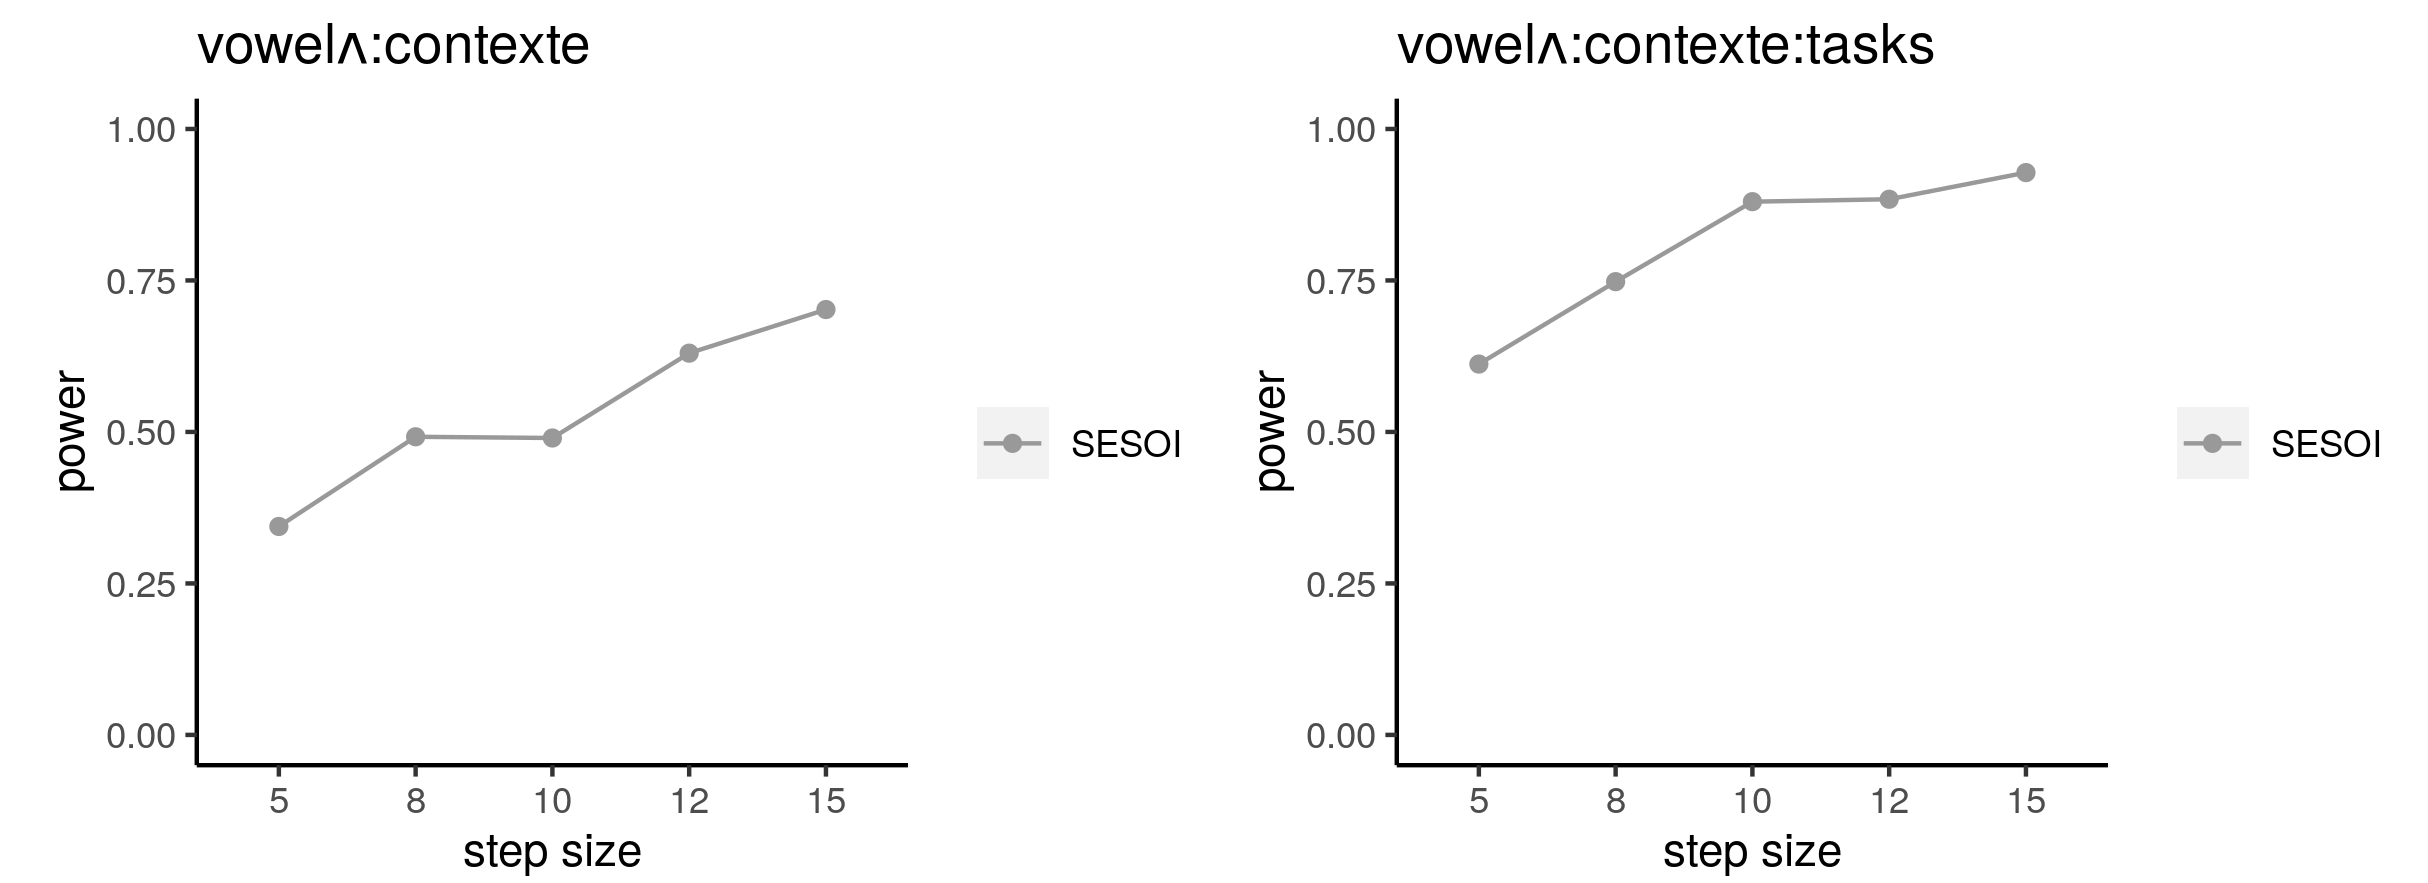
\includegraphics[width=\textwidth]{powerplot_f1_minus15} 
		\caption{Effect size = observed effect size - 15\%} \label{f1_minus15}
	\end{subfigure}
	
	\begin{subfigure}[t]{0.8\textwidth}
		\centering
		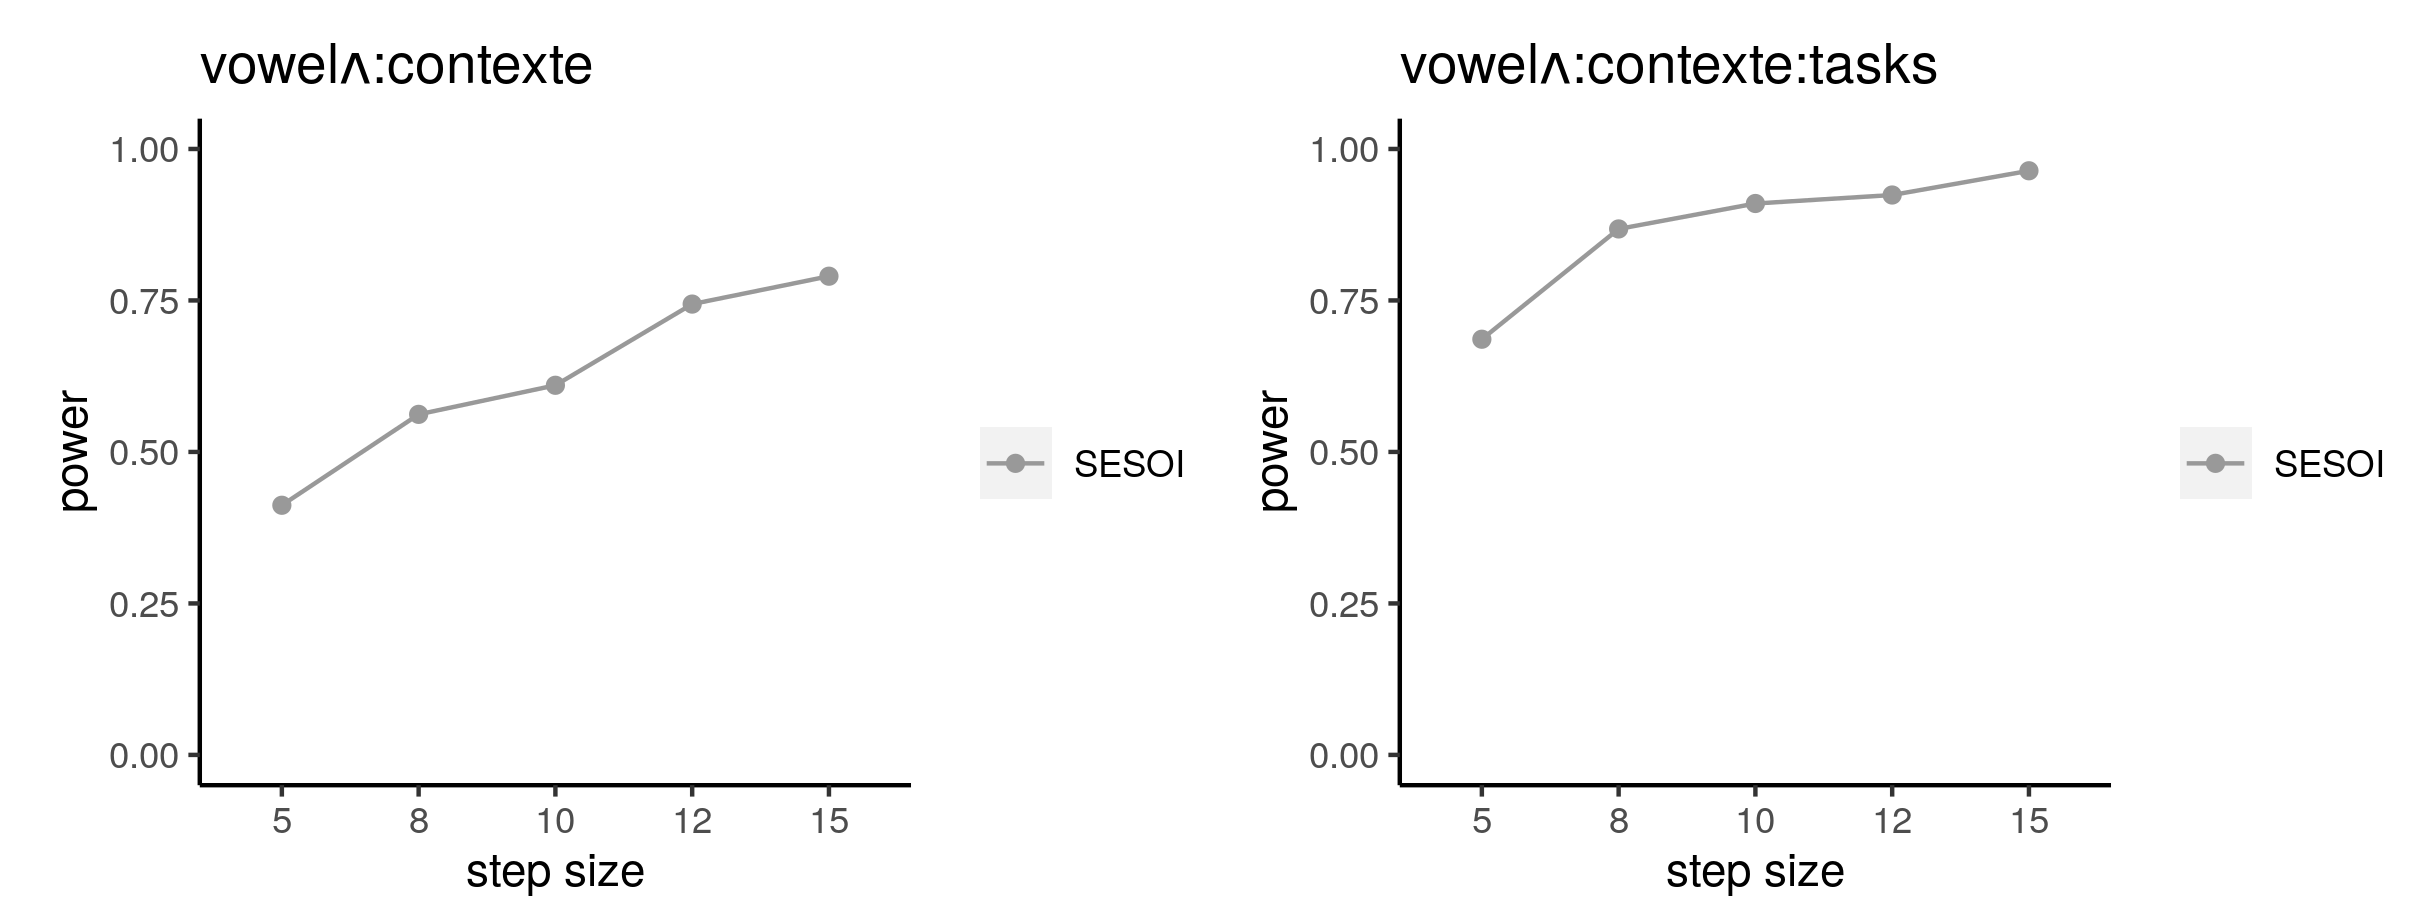
\includegraphics[width=\textwidth]{powerplot_f1_minus5} 
		\caption{Effect size = observed effect size - 5\%} \label{f1_minus5}
	\end{subfigure}
	
	
	\begin{subfigure}[t]{0.8\textwidth}
		\centering
		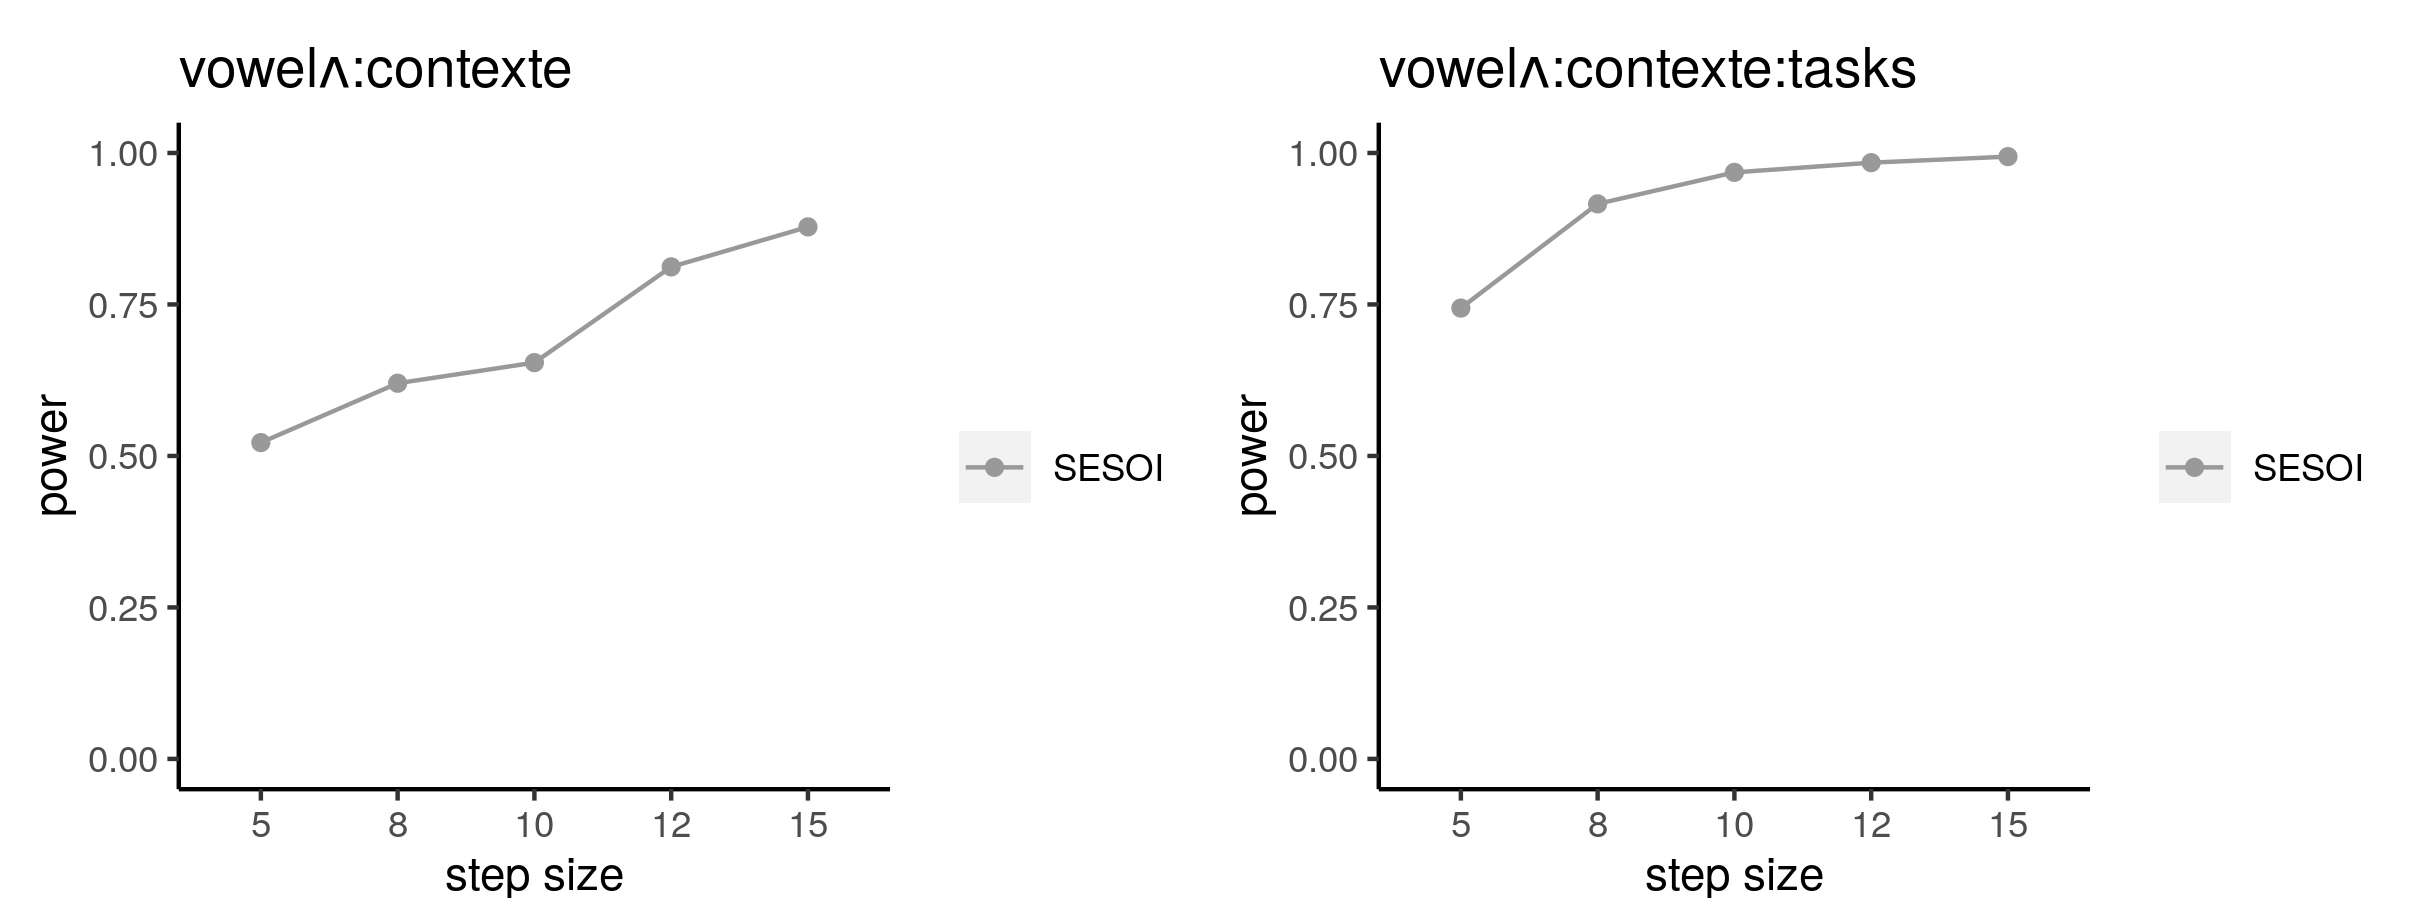
\includegraphics[width=\textwidth]{powerplot_f1_plus5} 
		\caption{Effect size = observed effect size + 5\%} \label{f1_plus5}
	\end{subfigure}
	
	
	\begin{subfigure}[t]{0.8\textwidth}
		\centering
		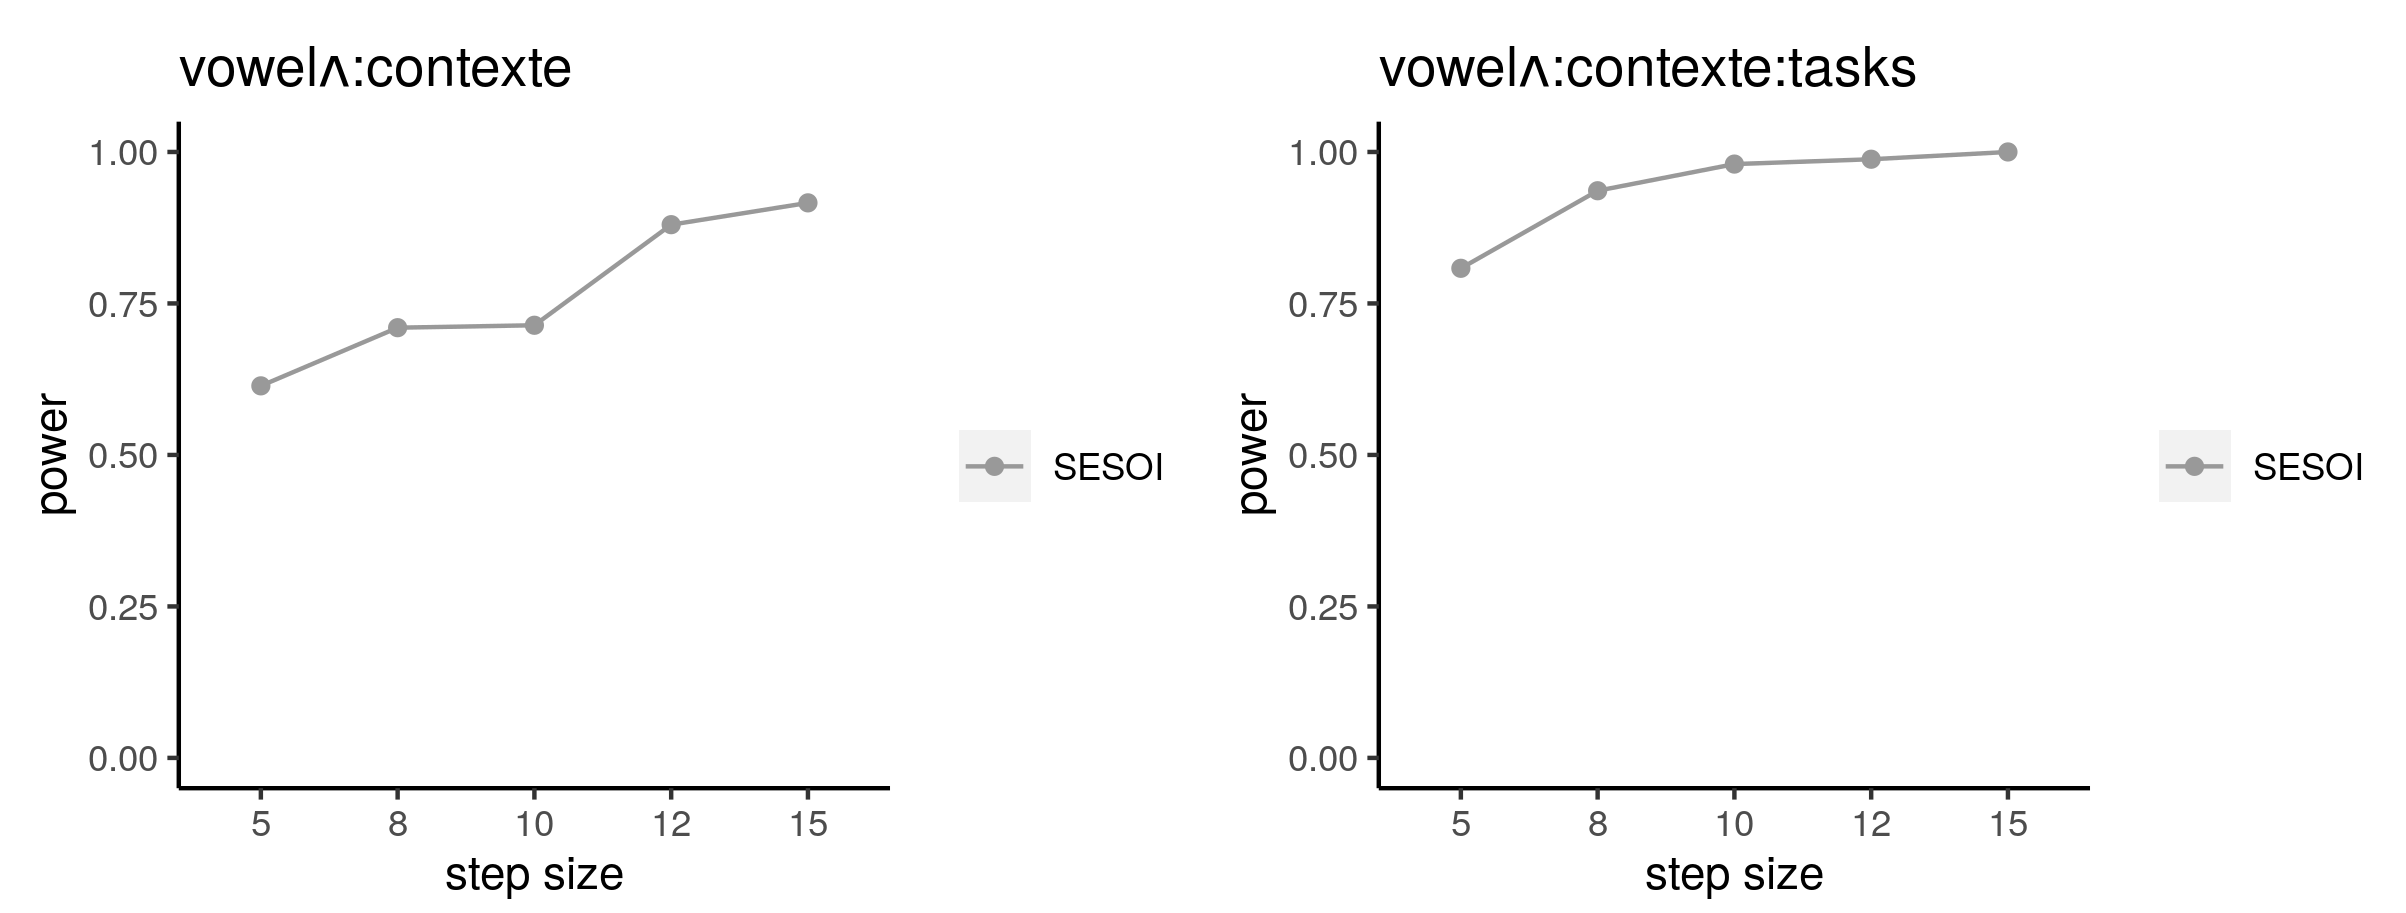
\includegraphics[width=\textwidth]{powerplot_f1_plus15} 
		\caption{Effect size = observed effect size + 15\%} \label{f1_plus15}
	\end{subfigure}
	
	\caption{Power analysis for fixed effects of interest at varying sample sizes: F1}
	
\end{figure}


\begin{figure}[!htb] \label{figure_power_analysis_f2}
	\centering
	\begin{subfigure}[t]{0.8\textwidth}
		\centering
		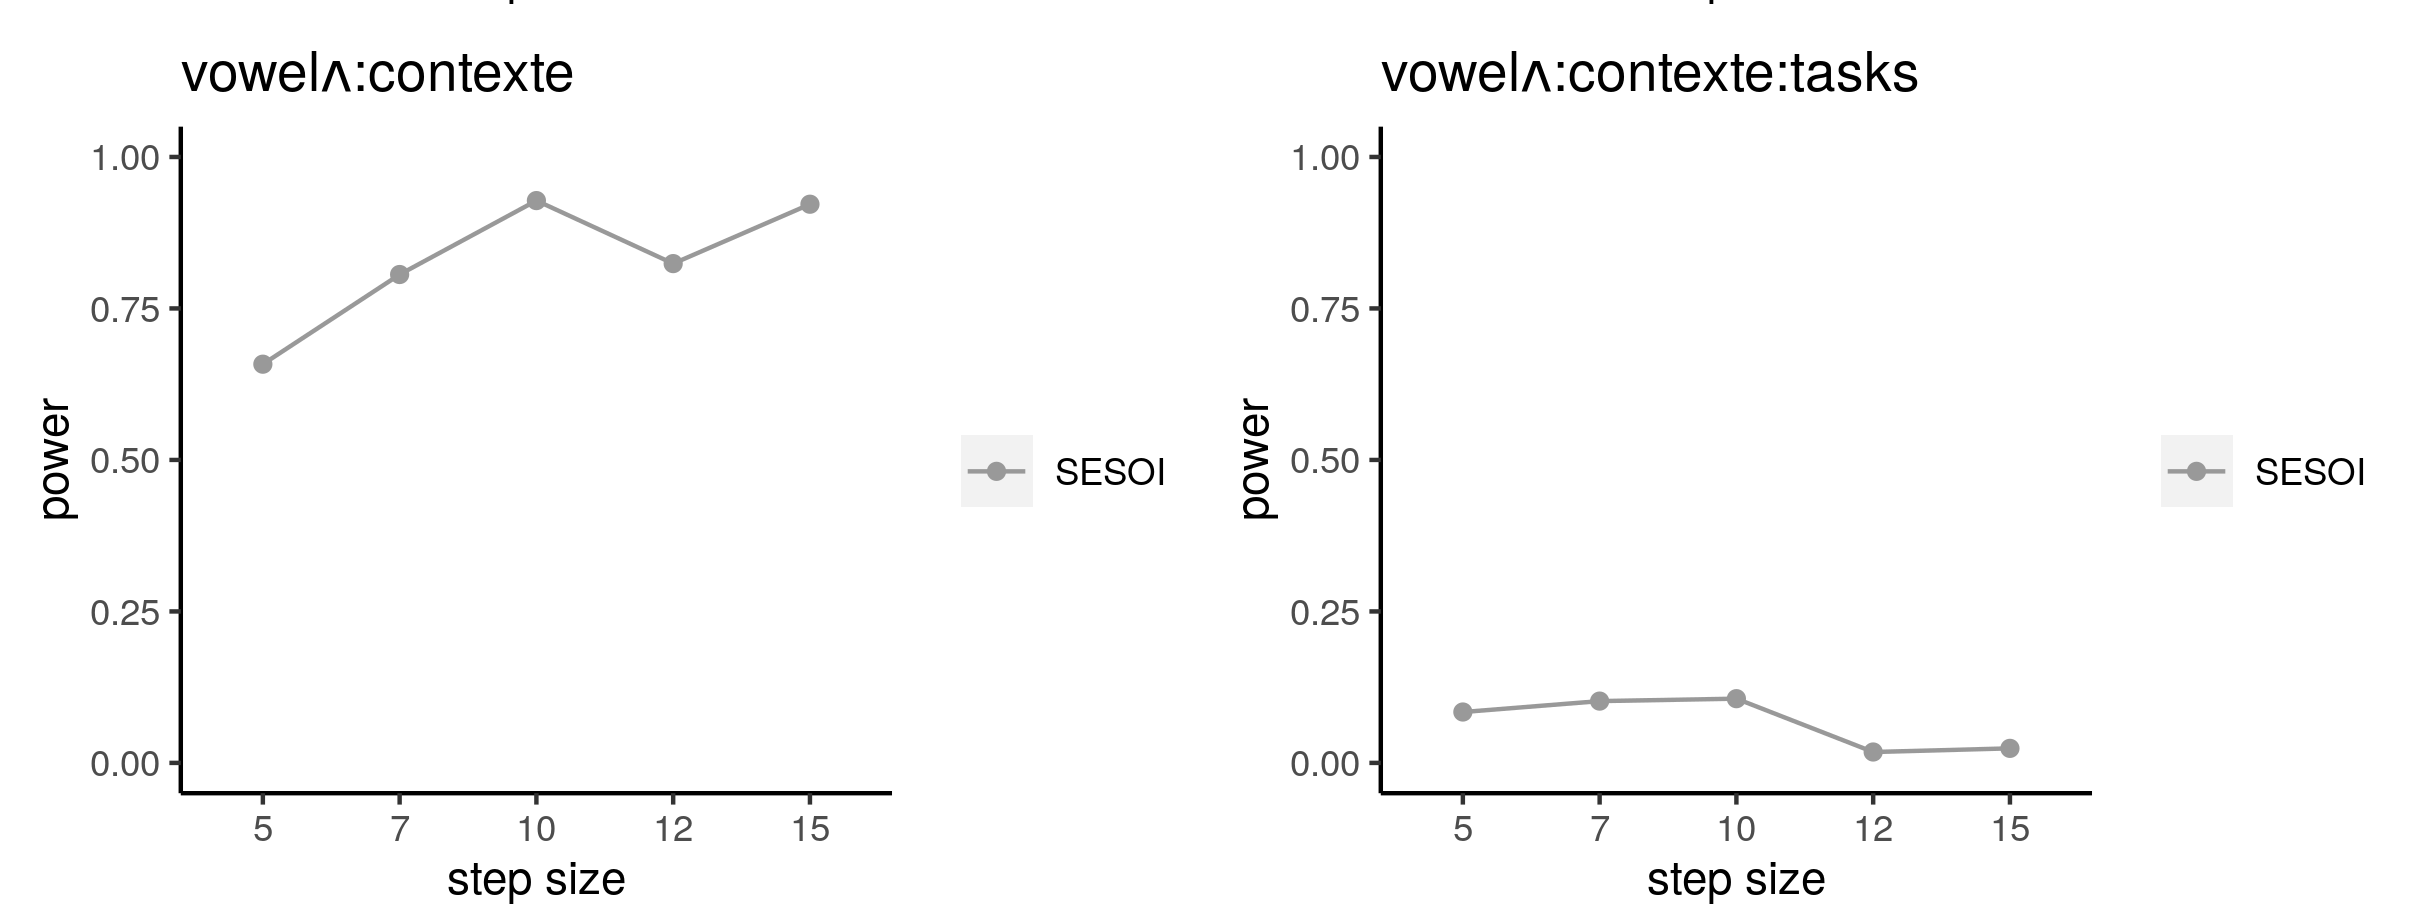
\includegraphics[width=\textwidth]{powerplot_f2_minus15} 
		\caption{Effect size = observed effect size - 15\%} \label{f2_minus15}
	\end{subfigure}
	
	\begin{subfigure}[t]{0.8\textwidth}
		\centering
		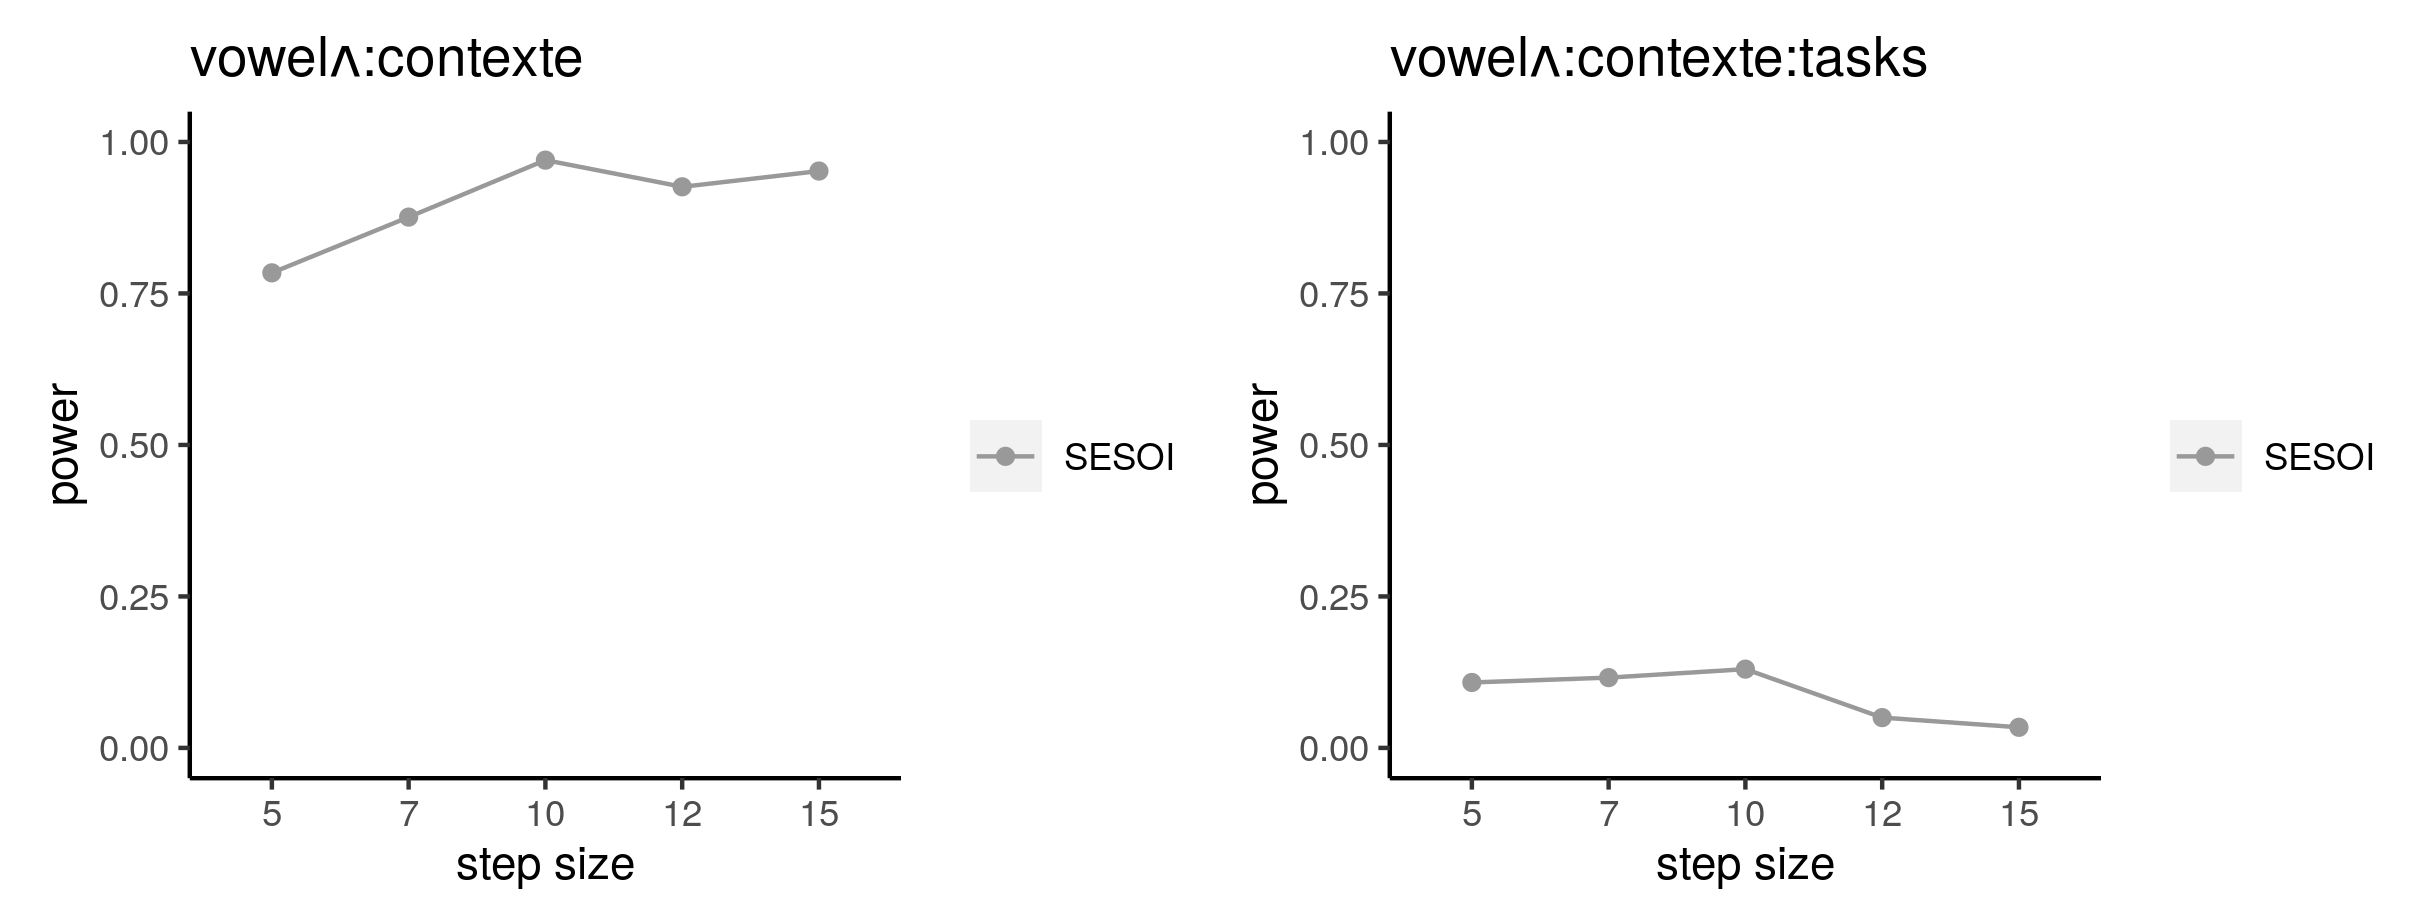
\includegraphics[width=\textwidth]{powerplot_f2_minus5} 
		\caption{Effect size = observed effect size - 5\%} \label{f2_minus5}
	\end{subfigure}
	
	
	\begin{subfigure}[t]{0.8\textwidth}
		\centering
		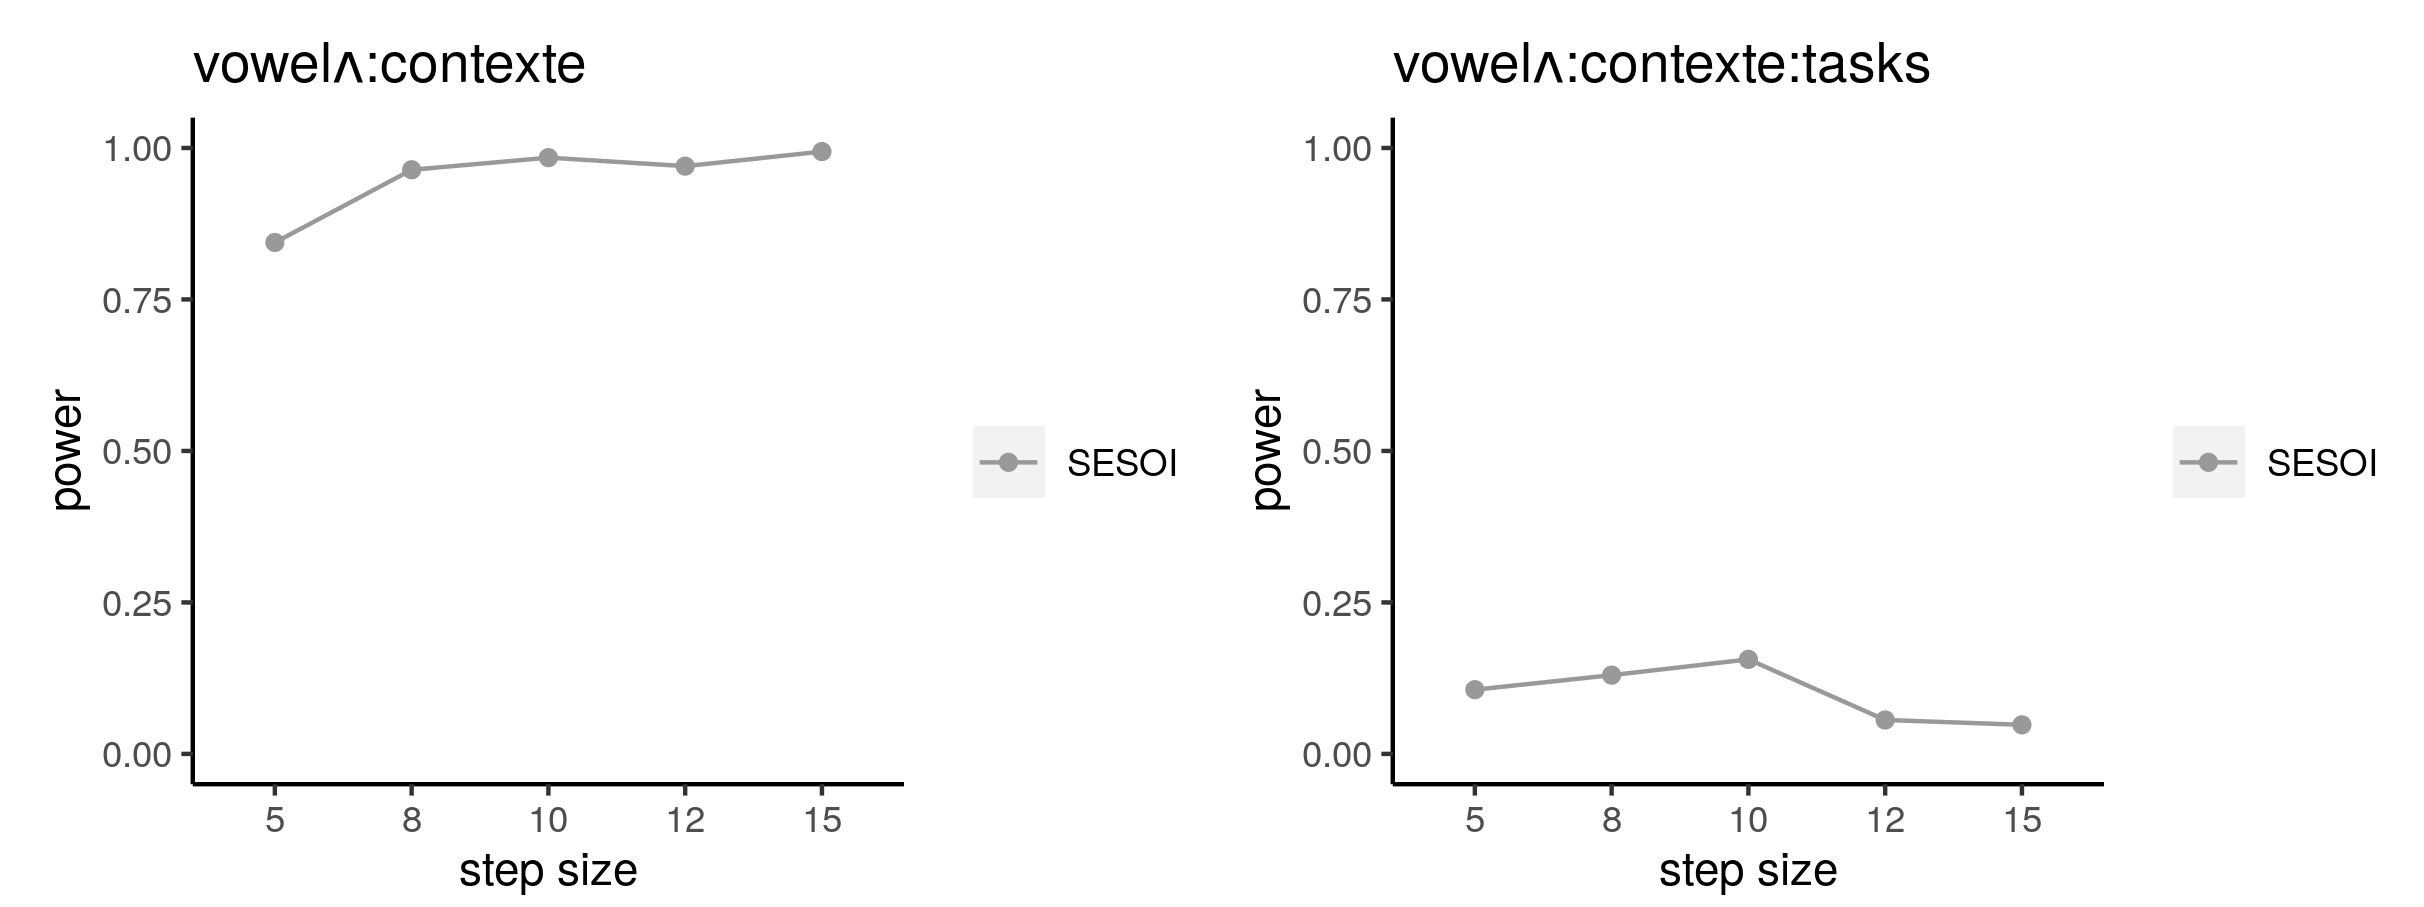
\includegraphics[width=\textwidth]{powerplot_f2_plus5} 
		\caption{Effect size = observed effect size + 5\%} \label{f2_plus5}
	\end{subfigure}
	
	
	\begin{subfigure}[t]{0.8\textwidth}
		\centering
		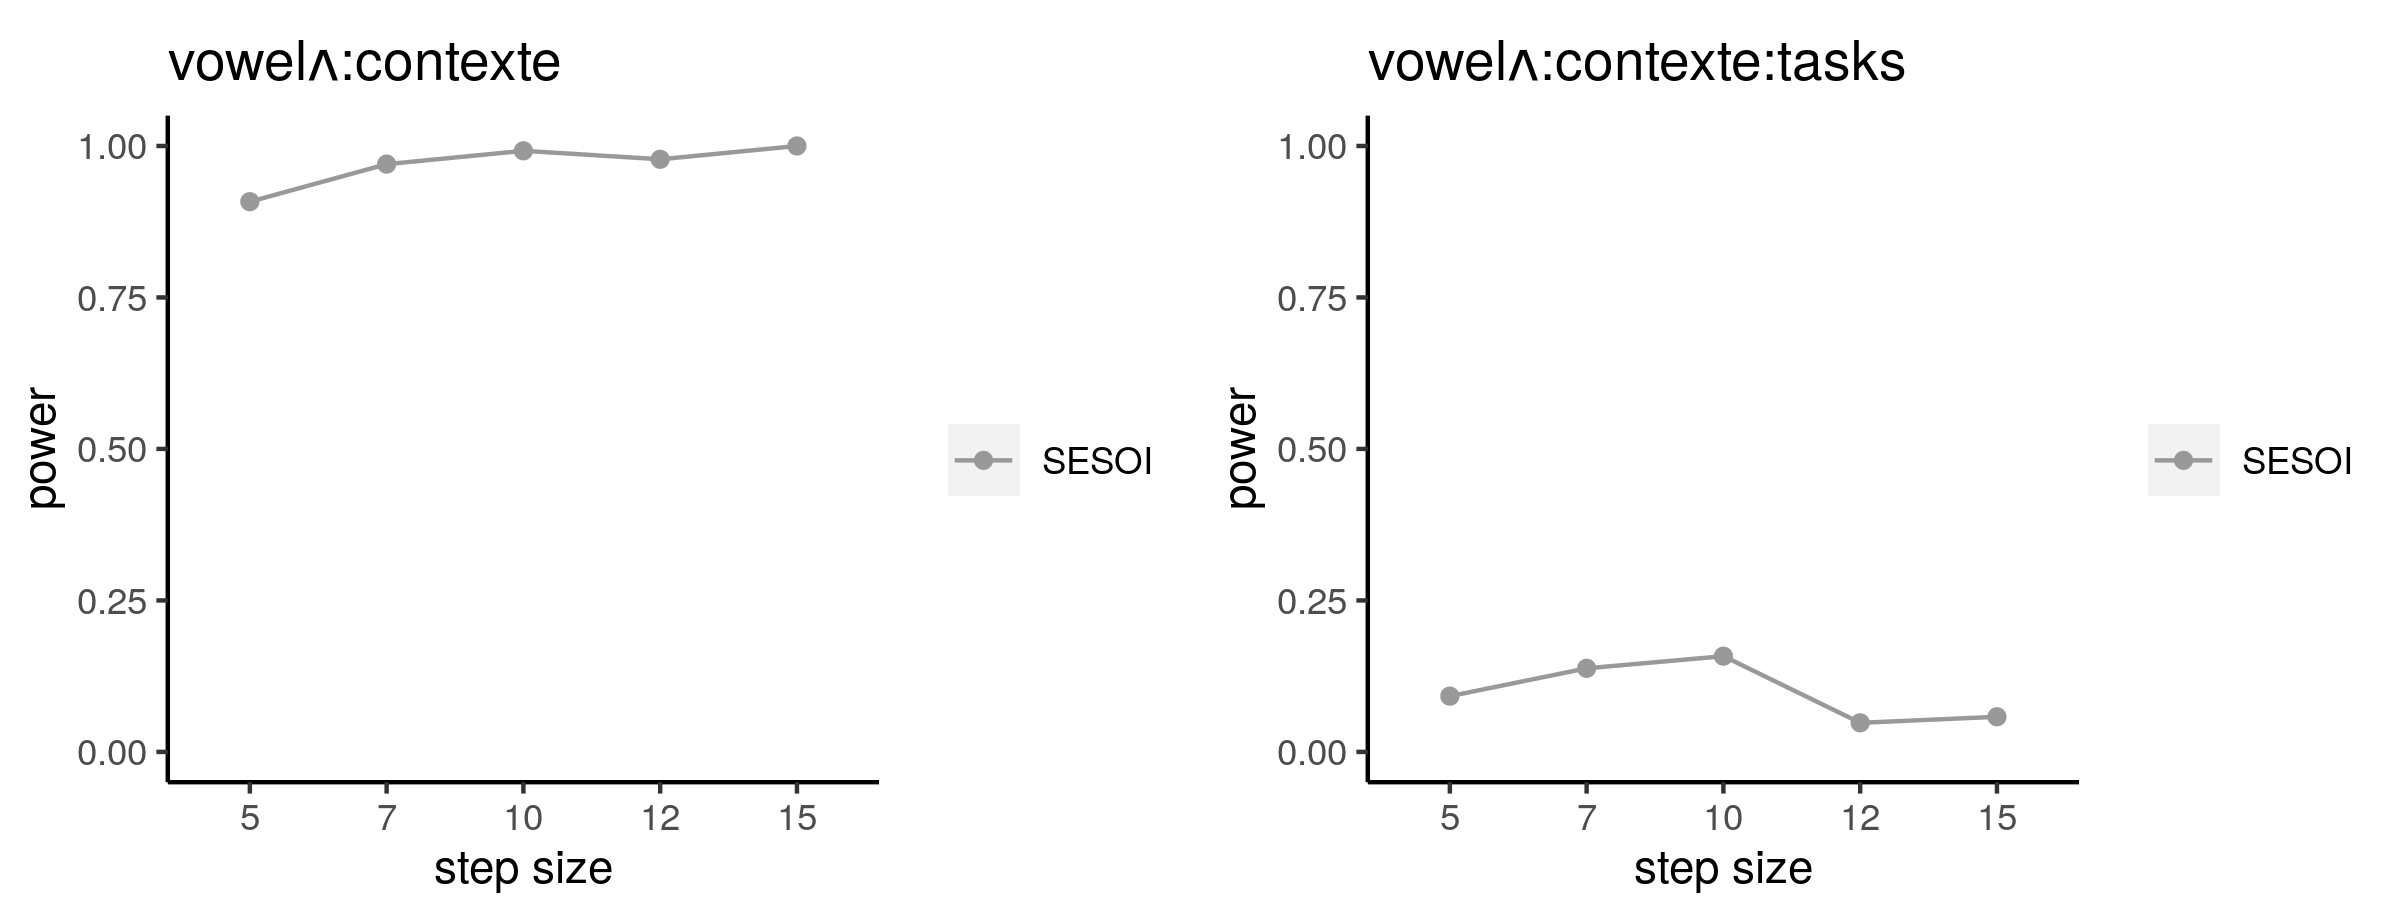
\includegraphics[width=\textwidth]{powerplot_f2_plus15} 
		\caption{Effect size = observed effect size + 15\%} \label{f2_plus15}
	\end{subfigure}
	
	\caption{Power analysis for fixed effects of interest at varying sample sizes: F2}
	
\end{figure}

\newpage


\subsubsection*{Baseline Bengali data from the SHRUTI corpus}

The SHRUTI corpus is the largest free corpus of Western Bengali speech that we are aware of. It comprises of 21.64 hours of read speech, containing 7383 unique sentences (22012 unique words) from Bengali newspapers in different domains, covering the most frequently used words of the language. The speakers are 34 adults (age range 20-40, 75\% male, 25\% female) who have grown up in the Indian state of West Bengal, and speak standard colloquial Bengali. All of the speakers have university-level education or higher. Given these parallels in linguistic, regional, and socio-economic background, we believe that Bengali speech from this corpus is representative of the average target Bengali vowel categories that are of interest in this study.
To estimate average vowel positions, we extracted formant values from syllable-initial productions of \nt{\ae} and \nt{a:}, at 55\% into the vowel, to get estimates from the steady state, which should most closely approximate the production target. Next, we compared these to our participants' productions in the non-switched English condition to understand the relative positions of these categories. This is visualized in figure \ref{vowels_unilingual_ie_bengali}. 

Note that we refrained from using corpus data for average Indian English vowel positions, opting instead to use the participant data from this study, because IE has high regional variability (c.f. discussion in section \ref{bengali_english_in_india}). To the best of our knowledge, there is no freely available corpus of IE speech from Bengali speakers in India. 


\clearpage
\bibliography{references}

\end{document}